\documentclass[12pt,letterpaper,oneside,reqno]{amsart}
\usepackage{amsfonts}
\usepackage{amsmath}
\usepackage{amssymb}
\usepackage{amsthm}
\usepackage{float}
\usepackage{mathrsfs}
\usepackage{colonequals}
\usepackage[font=small,labelfont=bf]{caption}
\usepackage[left=1in,right=1in,bottom=1in,top=1in]{geometry}
\usepackage[pdfpagelabels,hyperindex,colorlinks=true,linkcolor=blue,urlcolor=magenta,citecolor=green]{hyperref}
\usepackage{graphicx}
\linespread{1.7}
\emergencystretch=1em
\usepackage{array}
\usepackage{etoolbox}
\apptocmd{\sloppy}{\hbadness 10000\relax}{}{}
\raggedbottom

\newcommand \anglePower [2]{\langle #1 \rangle \sp{#2}}
\newcommand \bernoulli [2][B] {{#1}\sb{#2}}
\newcommand \curvePower [2]{\{#1\}\sp{#2}}
\newcommand \coeffA [3][A] {{\mathbf{#1}} \sb{#2,#3}}
\newcommand \polynomialP [4][P]{{\mathbf{#1}}\sp{#2} \sb{#3}(#4)}

% ordinary derivatives
\newcommand \derivative [2] {\frac{d}{d #2} #1}                              % 1 - function; 2 - variable;
\newcommand \pderivative [2] {\frac{\partial #1}{\partial #2}}               % 1 - function; 2 - variable;
\newcommand \qderivative [1] {D_{q} #1}                                      % 1 - function
\newcommand \nqderivative [1] {D_{n,q} #1}                                   % 1 - function
\newcommand \qpowerDerivative [1] {\mathcal{D}_q #1}                         % 1 - function;
\newcommand \finiteDifference [1] {\Delta #1}                                % 1 - function;
\newcommand \pTsDerivative [2] {\frac{\partial #1}{\Delta #2}}               % 1 - function; 2 - variable;

% high order derivatives
\newcommand \derivativeHO [3] {\frac{d^{#3}}{d {#2}^{#3}} #1}                % 1 - function; 2 - variable; 3 - order
\newcommand \pderivativeHO [3]{\frac{\partial^{#3}}{\partial {#2}^{#3}} #1}
\newcommand \qderivativeHO [2] {D_{q}^{#2} #1}                               % 1 - function; 2 - order
\newcommand \qpowerDerivativeHO [2] {\mathcal{D}_{q}^{#2} #1}                % 1 - function; 2 - order
\newcommand \finiteDifferenceHO [2] {\Delta^{#2} #1}                         % 1 - function; 2 - order
\newcommand \pTsDerivativeHO [3] {\frac{\partial^{#3}}{\Delta {#2}^{#3}} #1} % 1 - function; 2 - variable;

% central factorials and related symbols
\newcommand \centralFactorial [2] {#1^{[#2]}}
\newcommand \fallingFactorial [2] {\left(#1 \right)^{\underline{#2}}}
\newcommand{\stirlingii}{\genfrac{\{}{\}}{0pt}{}}
\newcommand{\eulerianNumber}{\genfrac{\langle}{\rangle}{0pt}{}}

% for llceil coeffcient
\newcommand{\nobarfrac}{\genfrac{}{}{0pt}{}}
\def\llceil{\left\lceil\kern-3.5pt\left\lceil}
\def\rrfloor{\right\rfloor\kern-3.5pt\right\rfloor}
\newcommand \llceilCoefficient [3] {\llceil \nobarfrac{#1}{#2} \rrfloor_{#3}}


\newtheorem{thm}{Theorem}[section]
\newtheorem{cor}[thm]{Corollary}
\newtheorem{lem}[thm]{Lemma}
\newtheorem{examp}[thm]{Example}
\newtheorem{conj}[thm]{Conjecture}
\newtheorem{defn}[thm]{Definition}

\numberwithin{equation}{section}

\title[LaTeX Template for Github]
{LaTeX Template for Github}
\author[Petro Kolosov]{Petro Kolosov}
\address{Software Developer, DevOps Engineer}
\email{kolosovp94@gmail.com}
\urladdr{https://kolosovpetro.github.io}
\keywords{
    Keyword1, Keyword2
}
\subjclass[2010]{26E70, 05A30}
\date{\today}
\hypersetup{
    pdftitle={LaTeX Template for Github},
    pdfsubject={
        Your Subject List
    },
    pdfauthor={Petro Kolosov},
    pdfkeywords={
        Your Keywords list
    }
}
\begin{document}
    \begin{abstract}
        In this manuscript, we show an odd-power identity in terms of certain matrix multiplication.
More precisely, the matrix of dimension $1 \times 1$ such that $a_{1,1} = N^{2M+1}$ is result of
multiplication of the three matrices $\unitMatrix{N} \times \matrixK{N}{M} \times \matrixT{M}$
\[
    \begin{bmatrix}
        N^{2M+1}
    \end{bmatrix} = \unitMatrix{N} \times \matrixK{N}{M} \times \matrixT{M}
\]
where $\unitMatrix{N}$ is unit row vector of dimension $1 \times N$; \quad
$\matrixK{N}{M}$ is a matrix of dimension $N \times M$,
and $\matrixT{M}$ is a column vector of size $M \times 1$.

    \end{abstract}

    \maketitle

    \tableofcontents


    \section{Introduction} \label{sec:introduction}
    Your introduction here.
Include some references~\cite{bayour2017truly,benkhettou2016conformable,caputo2009time,martins2009calculus,
    GithubSource_2022, Sloane_theencyclopedia}.
Lorem Ipsum is simply dummy text of the printing and typesetting industry.
Lorem Ipsum has been the industry's standard dummy text ever since the 1500s, when an unknown printer took a galley
of type and scrambled it to make a type specimen book.
It has survived not only five centuries, but also the leap into electronic typesetting, remaining essentially unchanged.
It was popularised in the 1960s with the release of Letraset sheets containing Lorem Ipsum passages, and more
recently with desktop publishing software like Aldus PageMaker including versions of Lorem Ipsum.

Figure example
\begin{figure}[H]
    \centering
    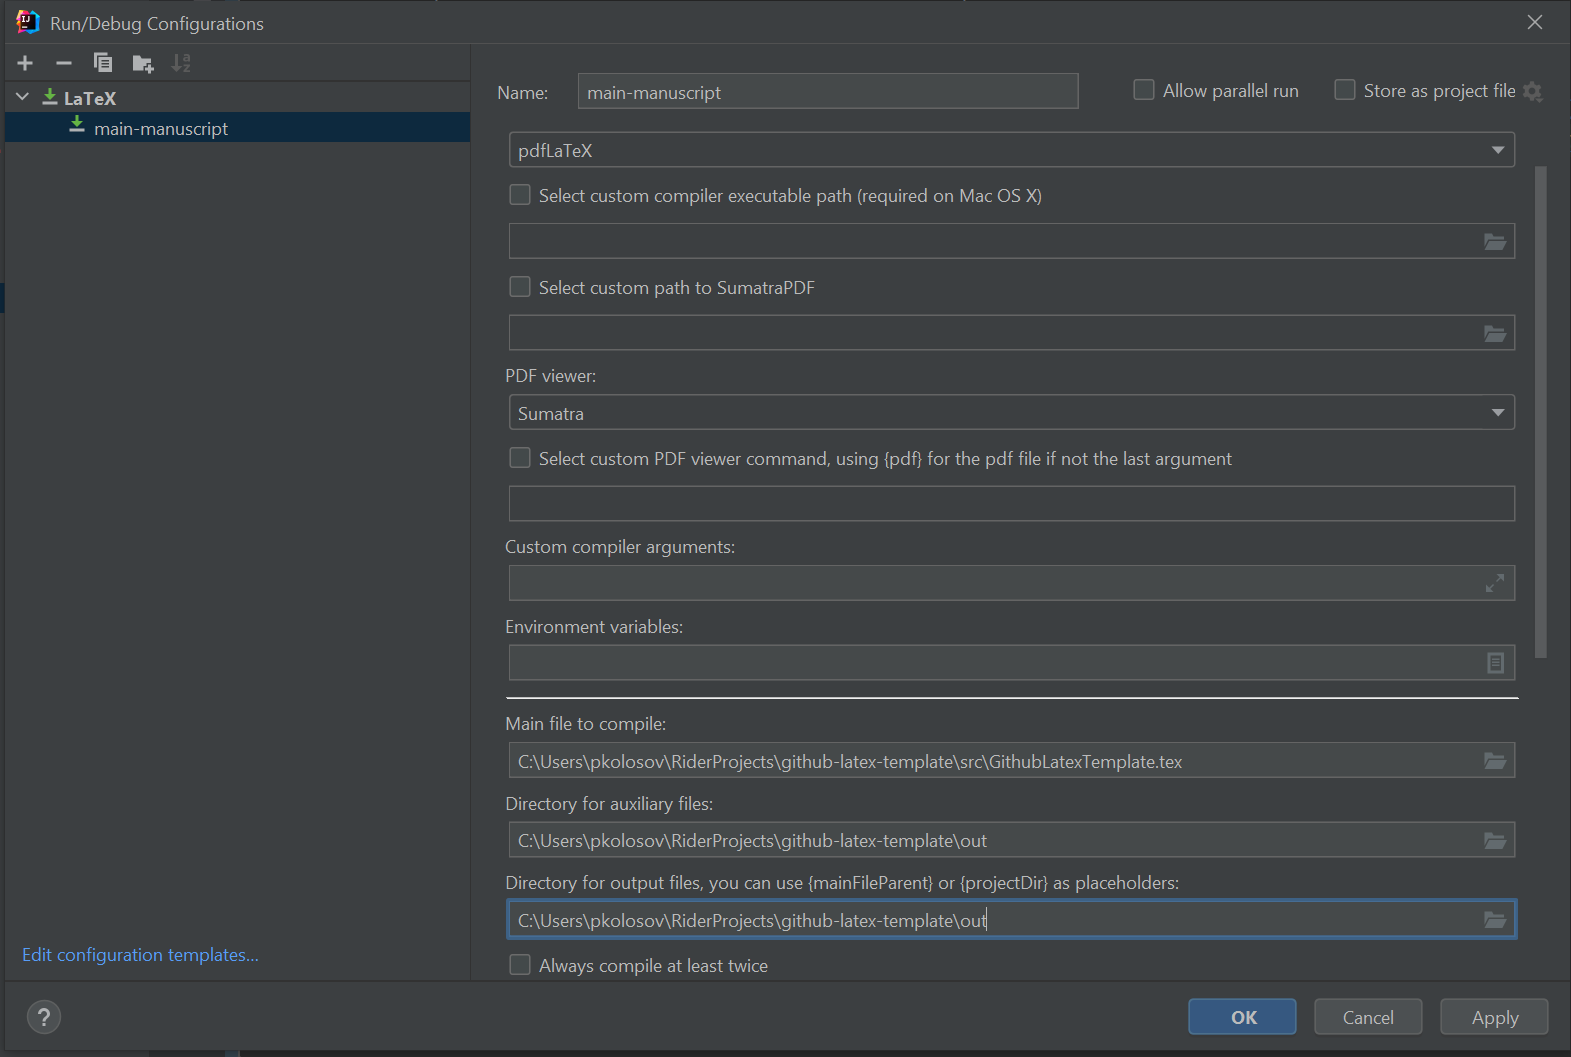
\includegraphics[width=1\textwidth]{../img/latex_configuration}
    ~\caption{Figure example.}\label{fig:figure}
\end{figure}

\begin{equation*}
     \llceil \nobarfrac{a}{b} \rrfloor_{m}
\end{equation*}
\begin{equation*}
    \llceilCoefficient{a}{b}{m}
\end{equation*}

And for any natural $m$ we have polynomial identity
\begin{equation}
    x^m = \sum_{k=1}^{m} T(m, k) \centralFactorial{x}{k}\label{eq:knuth-power-identity}
\end{equation}
where $\centralFactorial{x}{k}$ denotes central factorial defined by
\begin{equation*}
    \centralFactorial{x}{n} = x \fallingFactorial{x+\frac{n}{2}-1}{n-1}
\end{equation*}
where $\fallingFactorial{n}{k} = n (n-1) (n-2) \cdots (n-k+1)$ denotes falling factorial in Knuth's notation.
In particular,
\begin{equation*}
    \centralFactorial{x}{n}
    = x \left( x+\frac{n}{2}-1 \right) \left( x+\frac{n}{2}-1 \right) \cdots \left (x+\frac{n}{2}-n-1 \right)
    = x \prod_{k=1}^{n-1} \left( x+\frac{n}{2}-k \right)
\end{equation*}


    \section{Conclusions}\label{sec:conclusions}
    Conclusions of your manuscript.

    \bibliographystyle{unsrt}
    \bibliography{GithubLatexTemplate}
    \noindent \textbf{Version:} \texttt{Local-0.1.0}

\end{document}
